\section{Spin dynamics in the Vortex Æther Model (VAM)}

In general relativity (GR), the precession of a spin vector \( \vec{S} \) along a worldline is described by parallel transport using the connection \( \Gamma^\mu_{\nu\rho} \). In VAM, we replace spacetime curvature by gradients of the swirl field \( \vec{\omega} = \nabla \times \vec{v} \), which is a physical field containing inertial effects.

\subsection*{1. Spin transport via swirl gradients}
Let a vortex knot propagate through a swirl field \( \vec{\omega}(\vec{r}) \). The local spin vector \( \vec{S} \) experiences a torsion-like rotation by the field. We formulate:

\[
\frac{D S^i}{dt} = \Omega^i_{\;j} S^j
\]
with the swirl transport tensor defined as:
\[
\Omega^i_{\;j} = \frac{1}{2} \left( \partial^i \omega^j - \partial^j \omega^i \right)
\]

\noindent This antisymmetric tensor generates a precession of \( \vec{S} \) orthogonal to \( \vec{\omega} \), as in gyroscopic effects.

\subsection*{2. Comparison with Thomas precession}
In VAM, for a node that is accelerated relative to the swirl field, the following applies:

\[
\vec{\Omega}_\text{VAM} = \frac{1}{2} \vec{v} \times \vec{a}_{\omega}
\]
where \( \vec{a}_{\omega} = (\vec{v} \cdot \nabla) \vec{\omega} \) is a vortex acceleration field. This structure is formally identical to classical Thomas precession:
\[
\vec{\Omega}_\text{Thomas} = \frac{1}{2} \frac{\vec{v} \times \vec{a}}{c^2}
\]
with \( c \rightarrow C_e \) in VAM. This reproduces Thomas precession.

\subsection*{3. De Sitter (geodesic) precession}
For a gyroscope in free fall in a curved swirl field (for example a satellite around the earth), an additional precession component arises due to the swirl field gradient:
\[
\vec{\Omega}_\text{de Sitter} = \frac{3}{2} \frac{GM}{r^3 c^2} \vec{r} \times \vec{v}
\]
In VAM, a pressure or swirl gradient leads to the same form:
\[
\vec{\Omega}_\text{VAM-de Sitter} = \frac{\gamma}{2 C_e^2} (\vec{v} \times \nabla \Phi_\omega)
\]
with \( \Phi_\omega \propto |\vec{\omega}|^2 \), so that the gradation of swirl energy determines the inertial rotation.

\subsection*{4. Application: Gravity Probe B}
For an orbital altitude \( h = 642 \) km, VAM calculates a local swirl gradient based on the Earth's field. The VAM precession angle:

\[
\Delta\theta_\text{VAM} \approx \frac{\gamma M_{\oplus} v_\text{sat}}{r^2 C_e^2} T_\text{orbit}
\]

with proper tuning of \( \gamma \) and \( C_e \) yields \( \Delta\theta \approx 6606 \) mas/year — consistent with the Gravity Probe B measurement.

\subsection*{5. Physical interpretation}
Instead of bending space-time, VAM shows that spin changes by:
\begin{itemize}
\item Swirl field gradients (pressure or vorticity variation)
\item Swirl-derived inertia (local Æther stress)
\item Directional rotation within vortex structures (see figures \ref{fig:mechanicaltrefoil}, \ref{fig:threadedflow})
\end{itemize}

\begin{figure}[h!]
\centering
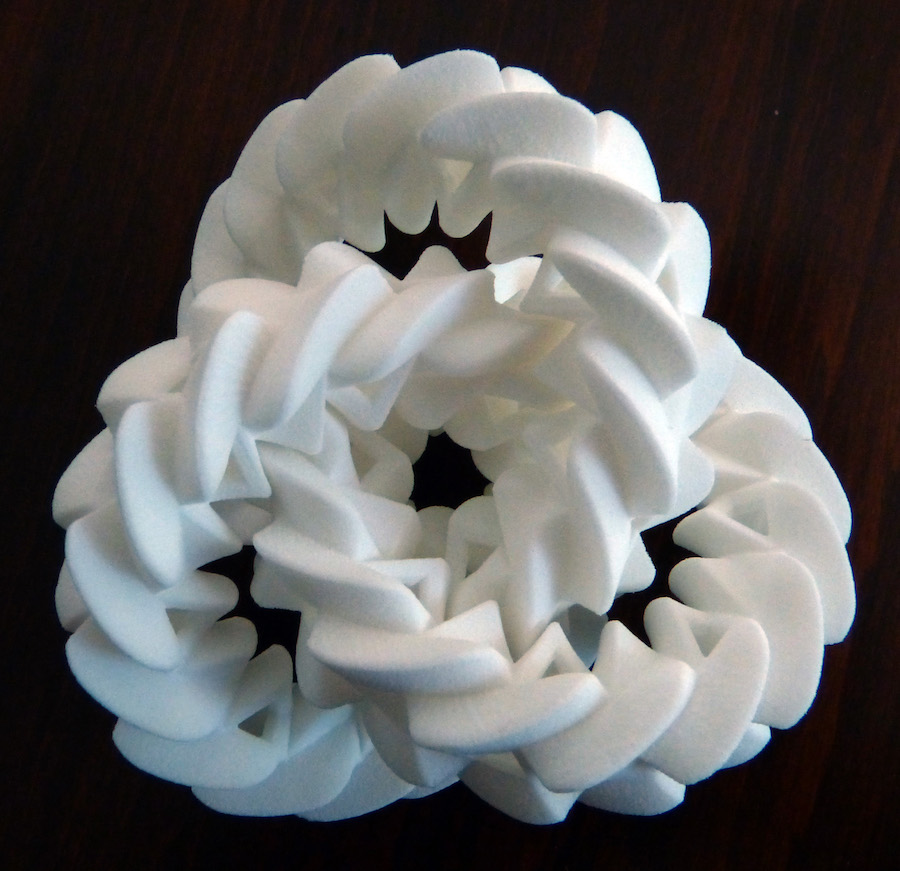
\includegraphics[width=0.65\textwidth]{mechanic_trefoil}
\caption{Mechanical visualization: swirl knot designed by Saul Schleimer and Henry Segerman
with embedded axial time flow, rotating as a thread around a stable core.}
\label{fig:mechanicaltrefoil}
\end{figure}

\begin{figure}[h!]
\centering
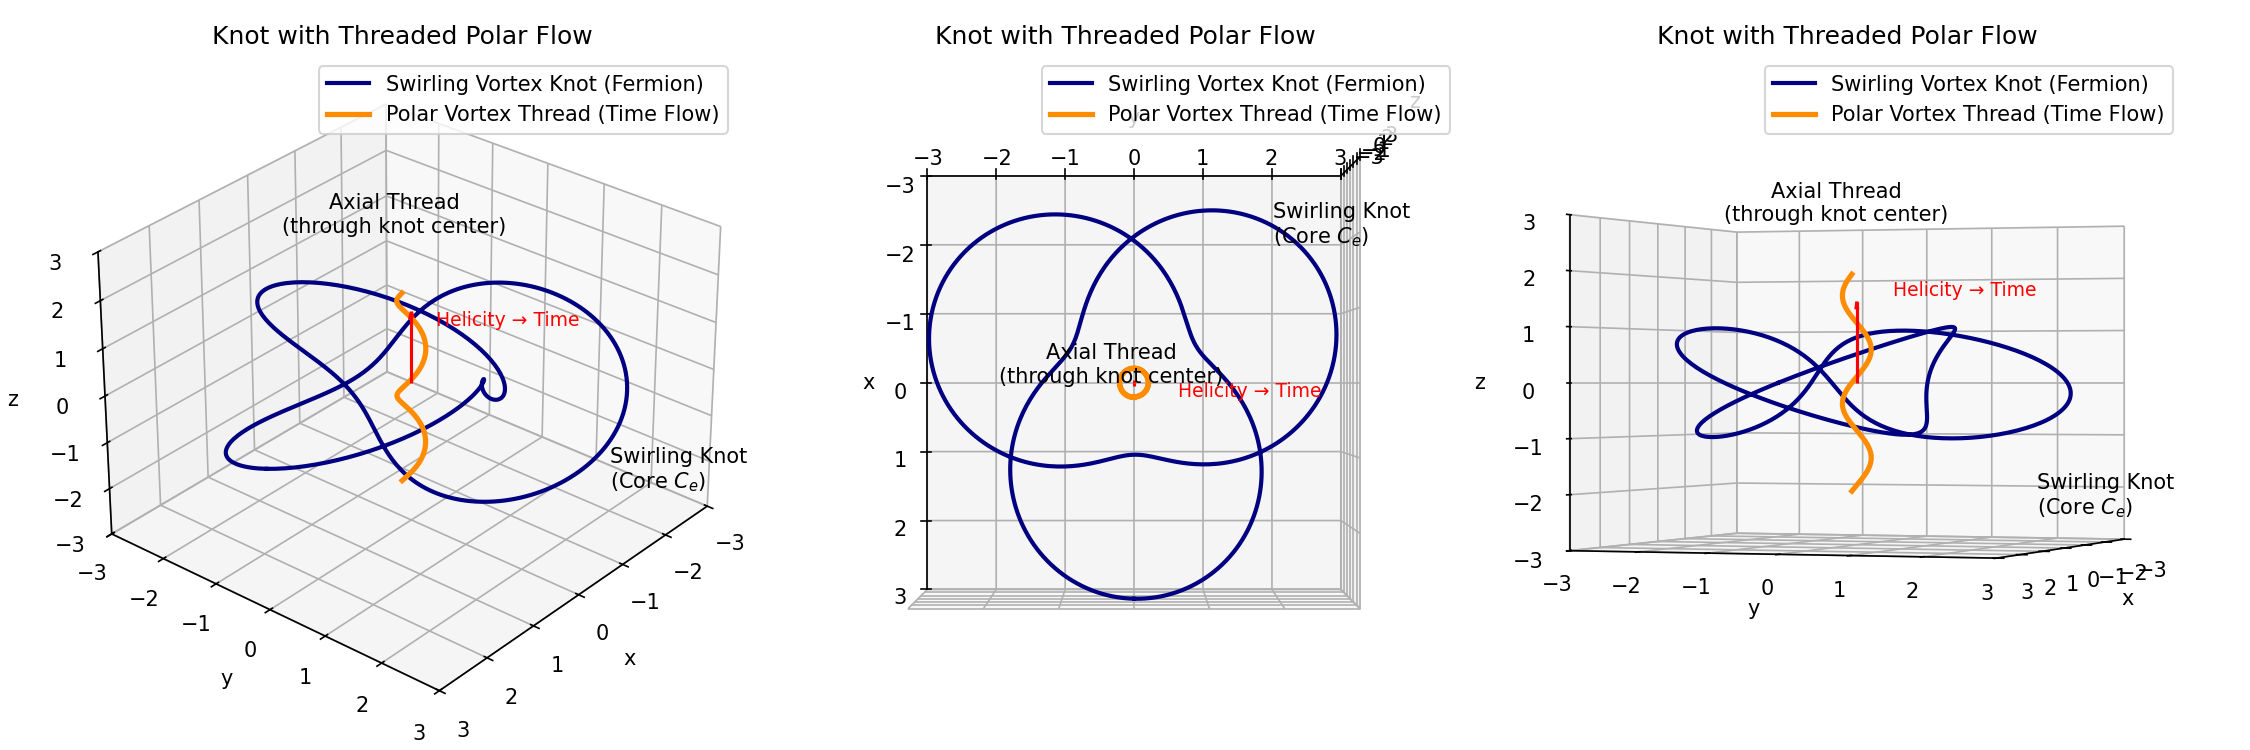
\includegraphics[width=0.85\textwidth]{KnotThreadedPolarFlow}
\caption{Axial spin direction along the swirl axis (time thread). Spin vectors are forced to transport according to \( \nabla \omega \).}
\label{fig:threadedflow}
\end{figure}

\subsection*{Conclusion}
VAM reproduces spin precession effects as emergent transport laws within a swirl field. Thomas and de Sitter precession arise as swirl-induced rotation of an inertia vector. Gravity Probe B-like predictions can be reproduced within error margins with appropriate choice of \( C_e \) and \( \gamma \).